\documentclass{book}

\usepackage{times,mathptmx}
\usepackage[pdftex]{graphicx}
\usepackage{pdflscape}

\usepackage{subcaption}
\usepackage{graphicx}
\usepackage{float}
\usepackage[section]{placeins}
\usepackage{fancyhdr}

\pagestyle{fancy}
\rhead{}
\lhead{}
\chead{Page \thepage}
\cfoot{Supplemental Information to Predecisional Draft Report}
%\renewcommand{\headrulewidth}{0.4pt}
\renewcommand{\footrulewidth}{0.4pt}

\usepackage{color}
\usepackage{amsmath}
\usepackage{multirow}
\definecolor{linknavy}{rgb}{0,0,0.50196}
\definecolor{linkred}{rgb}{1,0,0}
\definecolor{linkblue}{rgb}{0,0,1}

\usepackage{xr-hyper}
\usepackage[pdftex,
        colorlinks=true,
        urlcolor=linkblue,     % \href{...}{...} external (URL)
        citecolor=linkred,     % citation number colors
        linkcolor=linknavy,    % \ref{...} and \pageref{...}
        pdfproducer={pdflatex},
        pagebackref,
        pdfpagemode=UseNone,
        bookmarksopen=true,
        plainpages=false,
        verbose]{hyperref}

\setlength{\textwidth}{6.5in}
\setlength{\textheight}{9.0in}
\setlength{\topmargin}{0.in}
\setlength{\headheight}{0.in}
\setlength{\headsep}{0.1in}
\setlength{\parindent}{0.25in}
\setlength{\oddsidemargin}{0.0in}
\setlength{\evensidemargin}{0.0in}




\begin{document}

\bibliographystyle{unsrt}
\thispagestyle{empty}


\vspace*{0.75in}

\begin{center}
\begin{Large}
{\bf Preliminary Summary of Experimental Measurements} \\
{\bf Supplemental Information} \\
\end{Large}
\hspace{1in} \\
\end{center}

\begin{center}
\begin{large}
Predecisional Draft Report\\
Submitted to the 2021 MaCFP Condensed Phase Workshop \\
August 26, 2020 \\
\end{large}
\hspace{2in} \\
\end{center}

\begin{figure}[h]
  \centering
  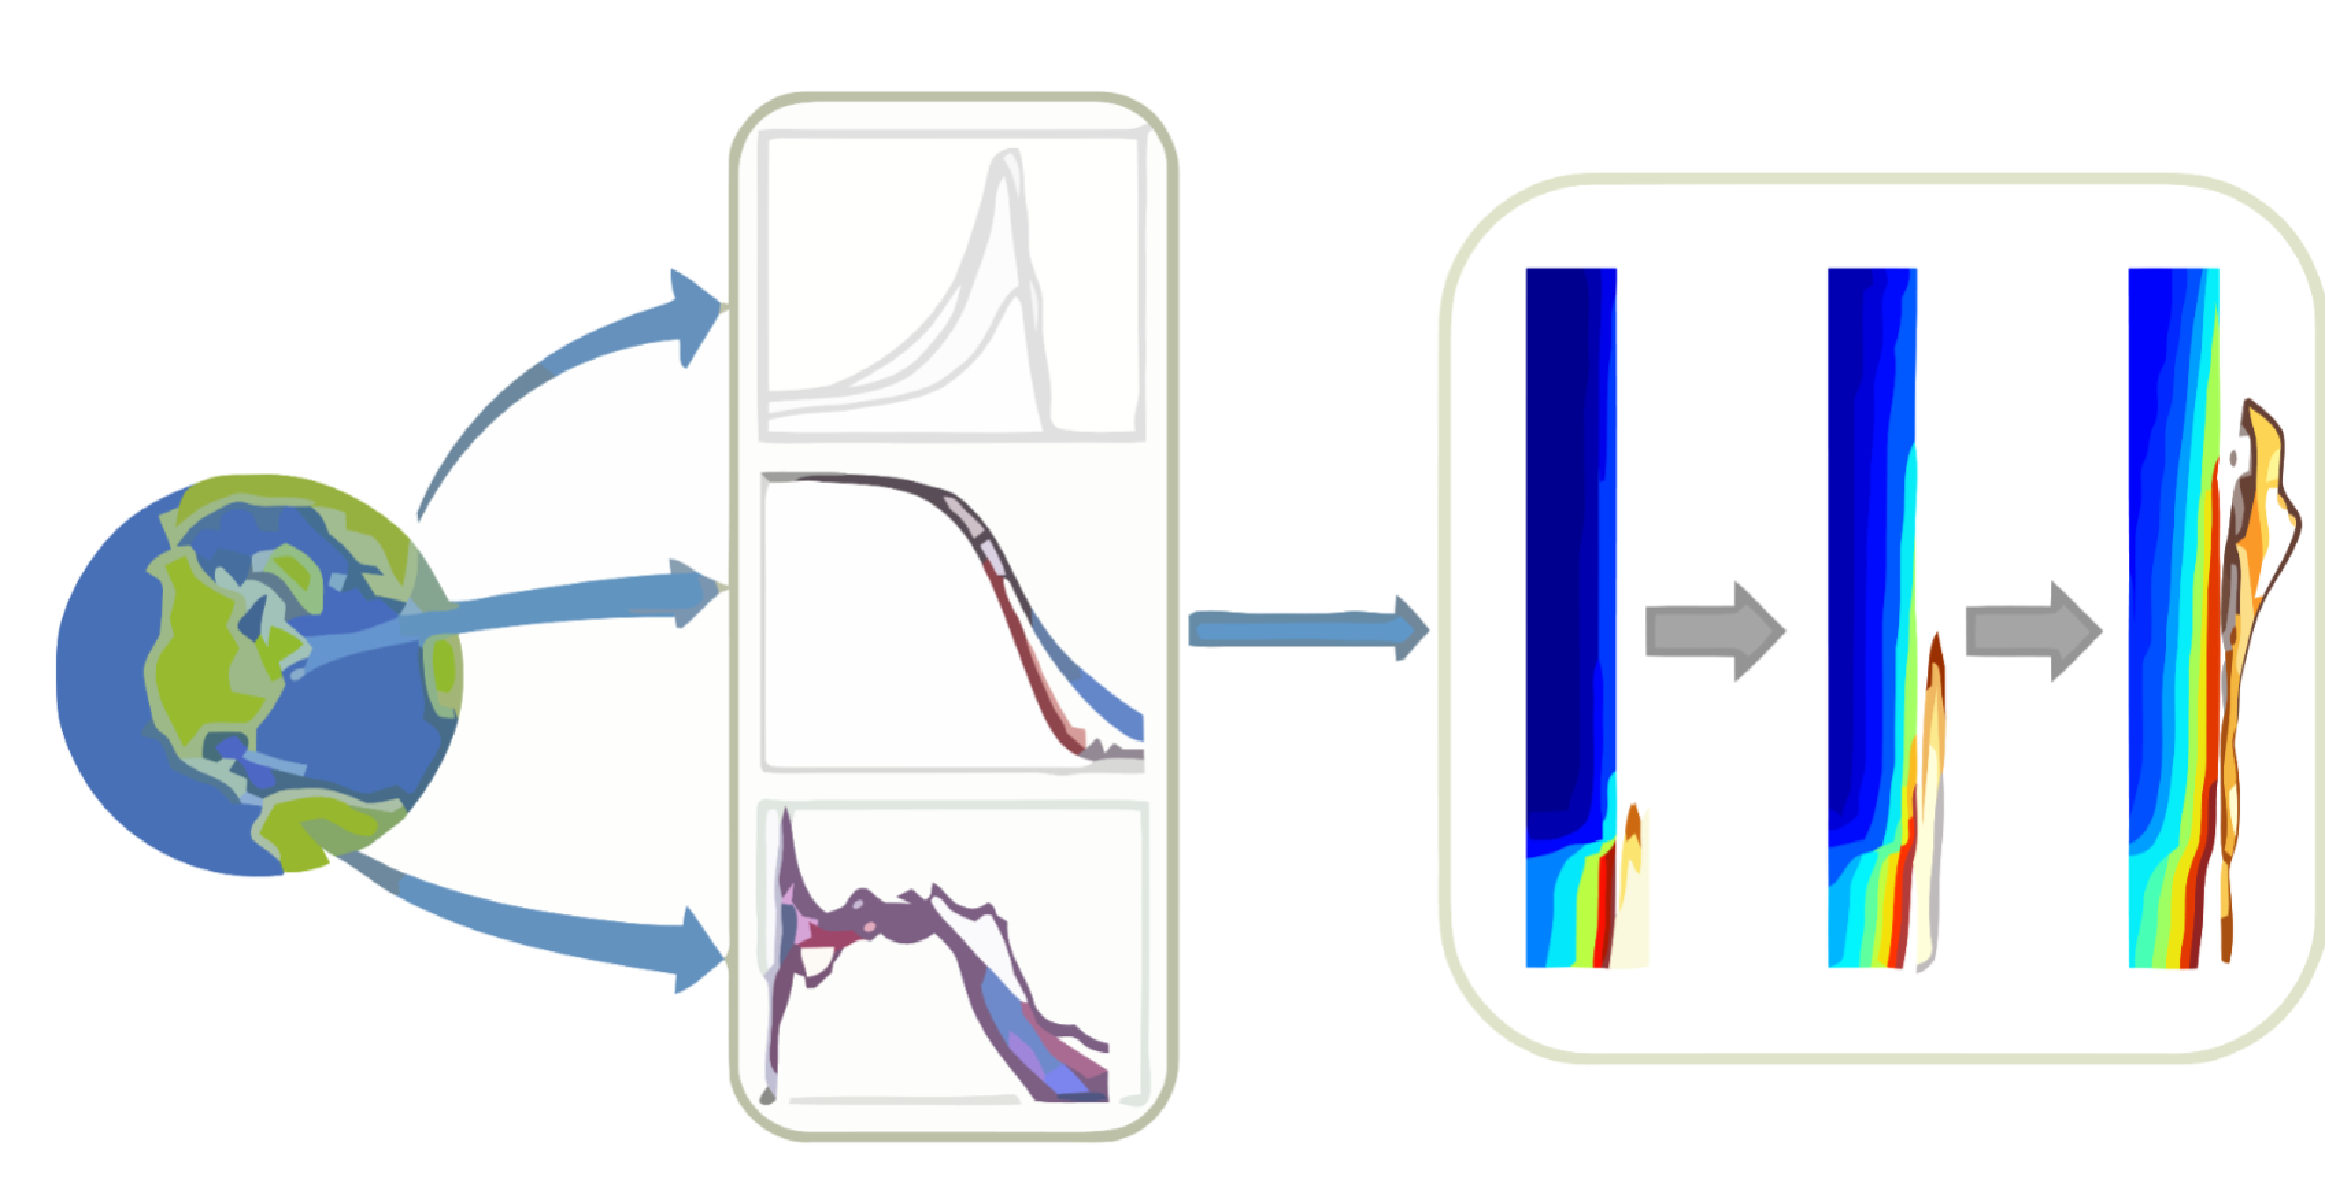
\includegraphics[width=6in]{FIGURES/MaCFP_Logo}
  \label{Cover_Image}
\end{figure}

\vfill

\begin{minipage}{0.25\textwidth}
\begin{figure}[H]

\includegraphics[width=2in]{FIGURES/IAFSSLogo}
\end{figure}
\end{minipage} \hfill
\begin{minipage}{0.7\textwidth}
\begin{flushright}
{\bf The MaCFP Condensed Phase Working Group Organizing Committee:} \\
Benjamin Batiot (University of Poitiers, France) \\
Morgan Bruns (Virginia Military Institute, USA) \\
Simo Hostikka (Aalto University, Finland) \\
Isaac Leventon (National Institute of Standards and Technology, USA) \\
Yuji Nakamura (Toyohashi University of Technology, Japan) \\
Pedro Reszka (Universidad Adolfo Ibáñez, Chile) \\
Thomas Rogaume (University of Poitiers, France) \\
Stanislav Stoliarov (University of Maryland, USA)
\end{flushright}
\end{minipage}


\newpage
\thispagestyle{empty}

\frontmatter


\chapter{Preface}

This Supplemental Information document has been prepared on behalf of the MaCFP Condensed Phase Working Group. It is written to provide supporting information to a predecisional draft report titled, `Preliminary Summary of Experimental Measurements'. All figures in this document have been prepared as described in the main (predecisional draft) report. These documents have been prepared for subject matter experts to provide critical review and to ensure the integrity of the measurement data and related analysis submitted to the 2021 MaCFP Condensed Phase Workshop. 

Parts of this work were prepared by the National Institute of Standards and Technology (NIST), an agency of the US government, and is not subject to copyright in the USA. Not all of the measurement data presented here has been through a formal review process. The identification of any commercial product or trade name does not imply endorsement or recommendation by NIST (or any other contributing institution). The policy of NIST is to use metric units of measurement in all its publications, and to provide statements of uncertainty for all original measurements. In this document, however, data from organizations outside NIST are shown, which may include measurements in non-metric units or measurements without uncertainty statements.

 

\newpage

\tableofcontents

\mainmatter

\pagestyle{fancy}



\begin{landscape}
\chapter{Thermogravimetric Analysis (TGA)}
\section{Nitrogen Environment}
\label{TGA_N2}
\subsection{$\beta$ = 1~K/min}
\begin{minipage}{0.65\textwidth}
\begin{figure}[H]
{\includegraphics[width=3.7in]{SCRIPT_FIGURES/UMET_TGA_N2_1K_avg}}\\
\end{figure}
\end{minipage}
\vfill
\newpage
\subsection{$\beta$ = 2~K/min}
\begin{minipage}{0.65\textwidth}
\begin{figure}[H]
{\includegraphics[width=3.7in]{SCRIPT_FIGURES/UMET_TGA_N2_2K_avg}}\\
\end{figure}
\end{minipage} 

\newpage
\subsection{$\beta$ = 5~K/min}
\begin{minipage}{0.65\textwidth}
\begin{figure}[H]
{\includegraphics[width=3.7in]{SCRIPT_FIGURES/LCPP_TGA_N2_5K_avg}}\\
\end{figure}
\end{minipage} 
\begin{minipage}{0.35\textwidth}
\begin{figure}[H]
{\includegraphics[width=3.7in]{SCRIPT_FIGURES/UMET_TGA_N2_5K_avg}}\\
\end{figure}
\end{minipage}

\newpage
\subsection{$\beta$ = 10~K/min}
\begin{minipage}{0.65\textwidth}
\begin{figure}[H]
{\includegraphics[width=3.7in]{SCRIPT_FIGURES/GIDAZE+_TGA_N2_10K_avg}}\\
\end{figure}
\end{minipage} 
\begin{minipage}{0.35\textwidth}
\begin{figure}[H]
{\includegraphics[width=3.7in]{SCRIPT_FIGURES/HKPoly_TGA_N2_10K_avg}}\\
\end{figure}
\end{minipage}\\
\begin{minipage}{0.65\textwidth}
\begin{figure}[H]
{\includegraphics[width=3.7in]{SCRIPT_FIGURES/LCPP_TGA_N2_10K_avg}}\\
\end{figure}
\end{minipage} 
\begin{minipage}{0.35\textwidth}
\begin{figure}[H]
{\includegraphics[width=3.7in]{SCRIPT_FIGURES/NIST_TGA_N2_10K_avg}}\\
\end{figure}
\end{minipage}\\
\begin{minipage}{0.65\textwidth}
\begin{figure}[H]
{\includegraphics[width=3.7in]{SCRIPT_FIGURES/TIFP_TGA_N2_10K_avg}}\\
\end{figure}
\end{minipage} 
\begin{minipage}{0.35\textwidth}
\begin{figure}[H]
{\includegraphics[width=3.7in]{SCRIPT_FIGURES/UClan_TGA_N2_10K_avg}}\\
\end{figure}
\end{minipage}\\
\begin{minipage}{0.65\textwidth}
\begin{figure}[H]
{\includegraphics[width=3.7in]{SCRIPT_FIGURES/UDRI_TGA_N2_10K_avg}}\\
\end{figure}
\end{minipage} 
\begin{minipage}{0.35\textwidth}
\begin{figure}[H]
{\includegraphics[width=3.7in]{SCRIPT_FIGURES/UMD_TGA_N2_10K_avg}}\\
\end{figure}
\end{minipage}\\
\begin{minipage}{0.65\textwidth}
\begin{figure}[H]
{\includegraphics[width=3.7in]{SCRIPT_FIGURES/UMET_TGA_N2_10K_avg}}\\
\end{figure}
\end{minipage} 
\begin{minipage}{0.35\textwidth}
\begin{figure}[H]
{\includegraphics[width=3.7in]{SCRIPT_FIGURES/UQ_TGA_N2_10K_avg}}\\
\end{figure}
\end{minipage}\\

\newpage
\subsection{$\beta$ = 15~K/min}
\begin{minipage}{0.65\textwidth}
\begin{figure}[H]
{\includegraphics[width=3.7in]{SCRIPT_FIGURES/LCPP_TGA_N2_15K_avg}}\\
\end{figure}
\end{minipage} 

\newpage
\subsection{$\beta$ = 20~K/min}
\begin{minipage}{0.65\textwidth}
\begin{figure}[H]
{\includegraphics[width=3.7in]{SCRIPT_FIGURES/DBI_Lund_TGA_N2_20K_avg}}\\
\end{figure}
\end{minipage} 
\begin{minipage}{0.35\textwidth}
\begin{figure}[H]
{\includegraphics[width=3.7in]{SCRIPT_FIGURES/LCPP_TGA_N2_20K_avg}}\\
\end{figure}
\end{minipage}\\
\begin{minipage}{0.65\textwidth}
\begin{figure}[H]
{\includegraphics[width=3.7in]{SCRIPT_FIGURES/UMET_TGA_N2_20K_avg}}\\
\end{figure}
\end{minipage} 

\newpage
\subsection{$\beta$ = 50~K/min}
\begin{minipage}{0.65\textwidth}
\begin{figure}[H]
{\includegraphics[width=3.7in]{SCRIPT_FIGURES/UMET_TGA_N2_50K_avg}}\\
\end{figure}
\end{minipage} 

\newpage
\subsection{$\beta$ = 100~K/min}
\begin{minipage}{0.65\textwidth}
\begin{figure}[H]
{\includegraphics[width=3.7in]{SCRIPT_FIGURES/UMET_TGA_N2_100K_avg}}\\
\end{figure}
\end{minipage} 
\vfill

\section{Argon Environment}
\label{TGA_Ar}
\subsection{$\beta$ = 1~K/min}
\begin{minipage}{0.65\textwidth}
\begin{figure}[H]
{\includegraphics[width=3.7in]{SCRIPT_FIGURES/Sandia_TGA_Ar_1K_avg}}\\
\end{figure}
\end{minipage} 
\vfill

\subsection{$\beta$ = 10~K/min}
\begin{minipage}{0.65\textwidth}
\begin{figure}[H]
{\includegraphics[width=3.7in]{SCRIPT_FIGURES/Sandia_TGA_Ar_10K_avg}}\\
\end{figure}
\end{minipage} 
\vfill

\subsection{$\beta$ = 50~K/min}
\begin{minipage}{0.65\textwidth}
\begin{figure}[H]
{\includegraphics[width=3.7in]{SCRIPT_FIGURES/Sandia_TGA_Ar_50K_avg}}\\
\end{figure}
\end{minipage} 
\vfill

\section{Oxygen Environment}
\label{TGA_O2}
\subsection{$X_{\rm O_2}=0.10$ $\beta$ = 10~K/min}
\begin{minipage}{0.65\textwidth}
\begin{figure}[H]
{\includegraphics[width=3.7in]{SCRIPT_FIGURES/GIDAZE+_TGA_O2-10_10K_avg}}\\
\end{figure}
\end{minipage} 
\vfill

\subsection{$X_{\rm O_2}=0.21$ $\beta$ = 10~K/min}
\begin{minipage}{0.65\textwidth}
\begin{figure}[H]
{\includegraphics[width=3.7in]{SCRIPT_FIGURES/GIDAZE+_TGA_O2-21_10K_avg}}\\
\end{figure}
\end{minipage} 
\begin{minipage}{0.35\textwidth}
\begin{figure}[H]
{\includegraphics[width=3.7in]{SCRIPT_FIGURES/HKPoly_TGA_O2-21_10K_avg}}\\
\end{figure}
\end{minipage}\\
\begin{minipage}{0.65\textwidth}
\begin{figure}[H]
{\includegraphics[width=3.7in]{SCRIPT_FIGURES/TIFP_TGA_O2-21_10K_avg}}\\
\end{figure}
\end{minipage} 
\begin{minipage}{0.35\textwidth}
\begin{figure}[H]
{\includegraphics[width=3.7in]{SCRIPT_FIGURES/UQ_TGA_O2-21_10K_avg}}\\
\end{figure}
\end{minipage}


\chapter{Differential Scanning Calorimetry (DSC)}
\section{Nitrogen Environment}
\label{DSC_N2}
\subsection{$\beta$ = 10~K/min}
\begin{minipage}{0.65\textwidth}
\begin{figure}[H]
{\includegraphics[width=3.7in]{SCRIPT_FIGURES/GIDAZE+_DSC_N2_10K_heatflow_avg}}\\
\end{figure}
\end{minipage}
\begin{minipage}{0.35\textwidth}
\begin{figure}[H]
{\includegraphics[width=3.7in]{SCRIPT_FIGURES/GIDAZE+_DSC_N2_10K_int_heatflow_avg}}\\
\end{figure}
\end{minipage}


\begin{minipage}{0.65\textwidth}
\begin{figure}[H]
{\includegraphics[width=3.7in]{SCRIPT_FIGURES/HKPoly_DSC_N2_10K_heatflow_avg}}\\
\end{figure}
\end{minipage}
\begin{minipage}{0.35\textwidth}
\begin{figure}[H]
{\includegraphics[width=3.7in]{SCRIPT_FIGURES/HKPoly_DSC_N2_10K_int_heatflow_avg}}\\
\end{figure}
\end{minipage}

\begin{minipage}{0.65\textwidth}
\begin{figure}[H]
{\includegraphics[width=3.7in]{SCRIPT_FIGURES/TIFP_DSC_N2_10K_heatflow_avg}}\\
\end{figure}
\end{minipage}
\begin{minipage}{0.35\textwidth}
\begin{figure}[H]
{\includegraphics[width=3.7in]{SCRIPT_FIGURES/TIFP_DSC_N2_10K_int_heatflow_avg}}\\
\end{figure}
\end{minipage}
\vfill

\begin{minipage}{0.65\textwidth}
\begin{figure}[H]
{\includegraphics[width=3.7in]{SCRIPT_FIGURES/UClan_DSC_N2_10K_heatflow_avg}}\\
\end{figure}
\end{minipage}
\begin{minipage}{0.35\textwidth}
\begin{figure}[H]
{\includegraphics[width=3.7in]{SCRIPT_FIGURES/UClan_DSC_N2_10K_int_heatflow_avg}}\\
\end{figure}
\end{minipage}

\begin{minipage}{0.65\textwidth}
\begin{figure}[H]
{\includegraphics[width=3.7in]{SCRIPT_FIGURES/UMD_DSC_N2_10K_heatflow_avg}}\\
\end{figure}
\end{minipage}
\begin{minipage}{0.35\textwidth}
\begin{figure}[H]
{\includegraphics[width=3.7in]{SCRIPT_FIGURES/UMD_DSC_N2_10K_int_heatflow_avg}}\\
\end{figure}
\end{minipage}
\vfill

\newpage
\subsection{$\beta$ = 20~K/min}
\begin{minipage}{0.65\textwidth}
\begin{figure}[H]
{\includegraphics[width=3.7in]{SCRIPT_FIGURES/DBI_Lund_DSC_N2_20K_heatflow_avg}}\\
\end{figure}
\end{minipage} 
\begin{minipage}{0.35\textwidth}
\begin{figure}[H]
{\includegraphics[width=3.7in]{SCRIPT_FIGURES/DBI_Lund_DSC_N2_20K_int_heatflow_avg}}\\
\end{figure}
\end{minipage}
\vfill

\newpage
\section{Argon Environment}
\label{DSC_Ar}
\subsection{$\beta$ = 1~K/min}
\begin{minipage}{0.65\textwidth}
\begin{figure}[H]
{\includegraphics[width=3.7in]{SCRIPT_FIGURES/Sandia_DSC_Ar_1K_heatflow_avg}}\\
\end{figure}
\end{minipage} 
\begin{minipage}{0.35\textwidth}
\begin{figure}[H]
{\includegraphics[width=3.7in]{SCRIPT_FIGURES/Sandia_DSC_Ar_1K_int_heatflow_avg}}\\
\end{figure}
\end{minipage}
\vfill

\subsection{$\beta$ = 10~K/min}
\begin{minipage}{0.65\textwidth}
\begin{figure}[H]
{\includegraphics[width=3.7in]{SCRIPT_FIGURES/Sandia_DSC_Ar_10K_heatflow_avg}}\\
\end{figure}
\end{minipage} 
\begin{minipage}{0.35\textwidth}
\begin{figure}[H]
{\includegraphics[width=3.7in]{SCRIPT_FIGURES/Sandia_DSC_Ar_10K_int_heatflow_avg}}\\
\end{figure}
\end{minipage}

\newpage
\subsection{$\beta$ = 50~K/min}
\begin{minipage}{0.65\textwidth}
\begin{figure}[H]
{\includegraphics[width=3.7in]{SCRIPT_FIGURES/Sandia_DSC_Ar_50K_heatflow_avg}}\\
\end{figure}
\end{minipage} 
\begin{minipage}{0.35\textwidth}
\begin{figure}[H]
{\includegraphics[width=3.7in]{SCRIPT_FIGURES/Sandia_DSC_Ar_50K_int_heatflow_avg}}\\
\end{figure}
\end{minipage}
\vfill

\newpage
\section{Oxygen Environment}
\label{DSC_O2}
\subsection{$X_{\rm O_2}=0.10$ $\beta$ = 10~K/min}
\begin{minipage}{0.65\textwidth}
\begin{figure}[H]
{\includegraphics[width=3.7in]{SCRIPT_FIGURES/GIDAZE+_DSC_O2-10_10K_heatflow_avg}}\\
\end{figure}
\end{minipage} 
\begin{minipage}{0.35\textwidth}
\begin{figure}[H]
{\includegraphics[width=3.7in]{SCRIPT_FIGURES/GIDAZE+_DSC_O2-10_10K_int_heatflow_avg}}\\
\end{figure}
\end{minipage}\\
\vfill

\subsection{$X_{\rm O_2}=0.21$ $\beta$ = 10~K/min}
\begin{minipage}{0.65\textwidth}
\begin{figure}[H]
{\includegraphics[width=3.7in]{SCRIPT_FIGURES/GIDAZE+_DSC_O2-21_10K_heatflow_avg}}\\
\end{figure}
\end{minipage} 
\begin{minipage}{0.35\textwidth}
\begin{figure}[H]
{\includegraphics[width=3.7in]{SCRIPT_FIGURES/GIDAZE+_DSC_O2-21_10K_int_heatflow_avg}}\\
\end{figure}
\end{minipage}\\
\begin{minipage}{0.65\textwidth}
\begin{figure}[H]
{\includegraphics[width=3.7in]{SCRIPT_FIGURES/HKPoly_DSC_O2-21_10K_heatflow_avg}}\\
\end{figure}
\end{minipage} 
\begin{minipage}{0.35\textwidth}
\begin{figure}[H]
{\includegraphics[width=3.7in]{SCRIPT_FIGURES/HKPoly_DSC_O2-21_10K_int_heatflow_avg}}\\
\end{figure}
\end{minipage}\\
\vfill
\begin{minipage}{0.65\textwidth}
\begin{figure}[H]
{\includegraphics[width=3.7in]{SCRIPT_FIGURES/TIFP_DSC_O2-21_10K_heatflow_avg}}\\
\end{figure}
\end{minipage} 
\begin{minipage}{0.35\textwidth}
\begin{figure}[H]
{\includegraphics[width=3.7in]{SCRIPT_FIGURES/TIFP_DSC_O2-21_10K_int_heatflow_avg}}\\
\end{figure}
\end{minipage}


\chapter{Cone Calorimeter}
\section{Heat Release Rate (HRR)}
\label{Cone_HRR}
\subsection{External heat flux: 25 kW/m$^2$}
\begin{minipage}{0.65\textwidth}
\begin{figure}[H]
{\includegraphics[width=3.7in]{SCRIPT_FIGURES/DBI_Lund_Cone_25kW_HRR}}\\
\end{figure}
\end{minipage}
\begin{minipage}{0.35\textwidth}
\begin{figure}[H]
{\includegraphics[width=3.7in]{SCRIPT_FIGURES/Edinburgh_Cone_25kW_HRR}}\\
\end{figure}
\end{minipage}\\
\vfill

\begin{minipage}{0.65\textwidth}
\begin{figure}[H]
{\includegraphics[width=3.7in]{SCRIPT_FIGURES/GIDAZE+_Cone_25kW_HRR}}\\
\end{figure}
\end{minipage}
\begin{minipage}{0.35\textwidth}
\begin{figure}[H]
{\includegraphics[width=3.7in]{SCRIPT_FIGURES/HKPoly_Cone_25kW_HRR}}\\
\end{figure}
\end{minipage}\\
\begin{minipage}{0.65\textwidth}
\begin{figure}[H]
{\includegraphics[width=3.7in]{SCRIPT_FIGURES/LCPP_Cone_25kW_HRR}}\\
\end{figure}
\end{minipage}
\begin{minipage}{0.35\textwidth}
\begin{figure}[H]
{\includegraphics[width=3.7in]{SCRIPT_FIGURES/NIST_Cone_25kW_HRR}}\\
\end{figure}
\end{minipage}
\vfill

\begin{minipage}{0.65\textwidth}
\begin{figure}[H]
{\includegraphics[width=3.7in]{SCRIPT_FIGURES/TIFP_Cone_25kW_HRR}}\\
\end{figure}
\end{minipage}
\begin{minipage}{0.35\textwidth}
\begin{figure}[H]
{\includegraphics[width=3.7in]{SCRIPT_FIGURES/UClan_Cone_25kW_HRR}}\\
\end{figure}
\end{minipage}\\

\begin{minipage}{0.65\textwidth}
\begin{figure}[H]
{\includegraphics[width=3.7in]{SCRIPT_FIGURES/UDRI_Cone_25kW_HRR}}\\
\end{figure}
\end{minipage}
\begin{minipage}{0.35\textwidth}
\begin{figure}[H]
{\includegraphics[width=3.7in]{SCRIPT_FIGURES/UQ_Cone_25kW_HRR}}\\
\end{figure}
\end{minipage}
\vfill


\newpage
\subsection{External heat flux: 50 kW/m$^2$}
\begin{minipage}{0.65\textwidth}
\begin{figure}[H]
{\includegraphics[width=3.7in]{SCRIPT_FIGURES/DBI_Lund_Cone_50kW_HRR}}\\
\end{figure}
\end{minipage}
\vfill

\newpage
\subsection{External heat flux: 65 kW/m$^2$}
\begin{minipage}{0.65\textwidth}
\begin{figure}[H]
{\includegraphics[width=3.7in]{SCRIPT_FIGURES/Aalto_Cone_65kW_HRR}}\\
\end{figure}
\end{minipage}
\begin{minipage}{0.35\textwidth}
\begin{figure}[H]
{\includegraphics[width=3.7in]{SCRIPT_FIGURES/DBI_Lund_Cone_65kW_HRR}}\\
\end{figure}
\end{minipage}\\
\begin{minipage}{0.65\textwidth}
\begin{figure}[H]
{\includegraphics[width=3.7in]{SCRIPT_FIGURES/Edinburgh_Cone_65kW_HRR}}\\
\end{figure}
\end{minipage}
\begin{minipage}{0.35\textwidth}
\begin{figure}[H]
{\includegraphics[width=3.7in]{SCRIPT_FIGURES/GIDAZE+_Cone_65kW_HRR}}\\
\end{figure}
\end{minipage}\\
\vfill 

\begin{minipage}{0.65\textwidth}
\begin{figure}[H]
{\includegraphics[width=3.7in]{SCRIPT_FIGURES/HKPoly_Cone_65kW_HRR}}\\
\end{figure}
\end{minipage}
\begin{minipage}{0.35\textwidth}
\begin{figure}[H]
{\includegraphics[width=3.7in]{SCRIPT_FIGURES/LCPP_Cone_65kW_HRR}}\\
\end{figure}
\end{minipage}\\
\begin{minipage}{0.65\textwidth}
\begin{figure}[H]
{\includegraphics[width=3.7in]{SCRIPT_FIGURES/TIFP_Cone_65kW_HRR}}\\
\end{figure}
\end{minipage}
\begin{minipage}{0.35\textwidth}
\begin{figure}[H]
{\includegraphics[width=3.7in]{SCRIPT_FIGURES/UClan_Cone_65kW_HRR}}\\
\end{figure}
\end{minipage}\\
\vfill 

\begin{minipage}{0.65\textwidth}
\begin{figure}[H]
{\includegraphics[width=3.7in]{SCRIPT_FIGURES/UDRI_Cone_65kW_HRR}}\\
\end{figure}
\end{minipage}
\begin{minipage}{0.35\textwidth}
\begin{figure}[H]
{\includegraphics[width=3.7in]{SCRIPT_FIGURES/UQ_Cone_65kW_HRR}}\\
\end{figure}
\end{minipage}\\
\vfill 

\newpage
\section{Surface Temperature}
\label{Cone_Temp}
\subsection{External heat flux: 25 kW/m$^2$}
\begin{minipage}{0.65\textwidth}
\begin{figure}[H]
{\includegraphics[width=3.7in]{SCRIPT_FIGURES/DBI_Lund_Cone_25kW_Temp}}\\
\end{figure}
\end{minipage}
\begin{minipage}{0.35\textwidth}
\begin{figure}[H]
{\includegraphics[width=3.7in]{SCRIPT_FIGURES/Edinburgh_Cone_25kW_Temp}}\\
\end{figure}
\end{minipage}
\vfill
\begin{minipage}{0.65\textwidth}
\begin{figure}[H]
{\includegraphics[width=3.7in]{SCRIPT_FIGURES/GIDAZE+_Cone_25kW_Temp}}\\
\end{figure}
\end{minipage}
\begin{minipage}{0.35\textwidth}
\begin{figure}[H]
{\includegraphics[width=3.7in]{SCRIPT_FIGURES/HKPoly_Cone_25kW_Temp}}\\
\end{figure}
\end{minipage}\\
\begin{minipage}{0.65\textwidth}
\begin{figure}[H]
{\includegraphics[width=3.7in]{SCRIPT_FIGURES/LCPP_Cone_25kW_Temp}}\\
\end{figure}
\end{minipage}
\begin{minipage}{0.35\textwidth}
\begin{figure}[H]
{\includegraphics[width=3.7in]{SCRIPT_FIGURES/TIFP_Cone_25kW_Temp}}\\
\end{figure}
\end{minipage}
\vfill

\begin{minipage}{0.65\textwidth}
\begin{figure}[H]
{\includegraphics[width=3.7in]{SCRIPT_FIGURES/UClan_Cone_25kW_Temp}}\\
\end{figure}
\end{minipage}
\begin{minipage}{0.35\textwidth}
\begin{figure}[H]
{\includegraphics[width=3.7in]{SCRIPT_FIGURES/UQ_Cone_25kW_Temp}}\\
\end{figure}
\end{minipage}
\vfill

\newpage
\subsection{External heat flux: 50 kW/m$^2$}
\begin{minipage}{0.65\textwidth}
\begin{figure}[H]
{\includegraphics[width=3.7in]{SCRIPT_FIGURES/Cone_50kW_TEMP}}\\
\end{figure}
\end{minipage}
\vfill

\newpage
\subsection{External heat flux: 65 kW/m$^2$}
\begin{minipage}{0.65\textwidth}
\begin{figure}[H]
{\includegraphics[width=3.7in]{SCRIPT_FIGURES/Aalto_Cone_65kW_Temp}}\\
\end{figure}
\end{minipage}
\begin{minipage}{0.35\textwidth}
\begin{figure}[H]
{\includegraphics[width=3.7in]{SCRIPT_FIGURES/DBI_Lund_Cone_65kW_Temp}}\\
\end{figure}
\end{minipage}

\begin{minipage}{0.65\textwidth}
\begin{figure}[H]
{\includegraphics[width=3.7in]{SCRIPT_FIGURES/Edinburgh_Cone_65kW_Temp}}\\
\end{figure}
\end{minipage}
\begin{minipage}{0.35\textwidth}
\begin{figure}[H]
{\includegraphics[width=3.7in]{SCRIPT_FIGURES/GIDAZE+_Cone_65kW_Temp}}\\
\end{figure}
\end{minipage}

\vfill

\begin{minipage}{0.65\textwidth}
\begin{figure}[H]
{\includegraphics[width=3.7in]{SCRIPT_FIGURES/HKPoly_Cone_65kW_Temp}}\\
\end{figure}
\end{minipage}
\begin{minipage}{0.35\textwidth}
\begin{figure}[H]
{\includegraphics[width=3.7in]{SCRIPT_FIGURES/LCPP_Cone_65kW_Temp}}\\
\end{figure}
\end{minipage}

\begin{minipage}{0.65\textwidth}
\begin{figure}[H]
{\includegraphics[width=3.7in]{SCRIPT_FIGURES/TIFP_Cone_65kW_Temp}}\\
\end{figure}
\end{minipage}
\begin{minipage}{0.35\textwidth}
\begin{figure}[H]
{\includegraphics[width=3.7in]{SCRIPT_FIGURES/UClan_Cone_65kW_Temp}}\\
\end{figure}
\end{minipage}
\vfill

\chapter{Anaerobic Gasification}
\section{Gasification Mass Flux}
\label{Gas_Mass}
\subsection{External heat flux: 25 kW/m$^2$}
\begin{minipage}{0.65\textwidth}
\begin{figure}[H]
{\includegraphics[width=3.7in]{SCRIPT_FIGURES/DBI_Lund_Gasification_25kW_smoothed}}\\
\end{figure}
\end{minipage}
\begin{minipage}{0.35\textwidth}
\begin{figure}[H]
{\includegraphics[width=3.7in]{SCRIPT_FIGURES/FM_FPA_25kW_smoothed}}\\
\end{figure}
\end{minipage}\\
\begin{minipage}{0.65\textwidth}
\begin{figure}[H]
{\includegraphics[width=3.7in]{SCRIPT_FIGURES/GIDAZE+_FPA_25kW_smoothed}}\\
\end{figure}
\end{minipage}
\vfill

\newpage
\subsection{External heat flux: 50 kW/m$^2$}
\begin{minipage}{0.65\textwidth}
\begin{figure}[H]
{\includegraphics[width=3.7in]{SCRIPT_FIGURES/DBI_Lund_Gasification_50kW_smoothed}}\\
\end{figure}
\end{minipage}
\begin{minipage}{0.35\textwidth}
\begin{figure}[H]
{\includegraphics[width=3.7in]{SCRIPT_FIGURES/FM_FPA_50kW_smoothed}}\\
\end{figure}
\end{minipage}\\
\vfill
\newpage
\subsection{External heat flux: 65 kW/m$^2$}
\begin{minipage}{0.65\textwidth}
\begin{figure}[H]
{\includegraphics[width=3.7in]{SCRIPT_FIGURES/Aalto_Gasification_65kW_smoothed}}\\
\end{figure}
\end{minipage}
\begin{minipage}{0.35\textwidth}
\begin{figure}[H]
{\includegraphics[width=3.7in]{SCRIPT_FIGURES/FM_FPA_65kW_smoothed}}\\
\end{figure}
\end{minipage}\\
\begin{minipage}{0.65\textwidth}
\begin{figure}[H]
{\includegraphics[width=3.7in]{SCRIPT_FIGURES/GIDAZE+_FPA_65kW_smoothed}}\\
\end{figure}
\end{minipage}
\begin{minipage}{0.35\textwidth}
\begin{figure}[H]
{\includegraphics[width=3.7in]{SCRIPT_FIGURES/TIFP_Gasification_65kW_smoothed}}\\
\end{figure}
\end{minipage}\\

\newpage
\section{Surface Temperature}
\label{Gas_Temp}
\subsection{External heat flux: 25 kW/m$^2$}
\begin{minipage}{0.65\textwidth}
\begin{figure}[H]
{\includegraphics[width=3.7in]{SCRIPT_FIGURES/GIDAZE+_FPA_25kW_Temp}}\\
\end{figure}
\end{minipage}

\begin{minipage}{0.35\textwidth}
\begin{figure}[H]
{\includegraphics[width=3.7in]{SCRIPT_FIGURES/FM_FPA_25kW_Temp}}\\
\end{figure}
\end{minipage}\\
‘Charlottetown’:  FPA ($\dot{q}_{\rm ext}'' = 25$~kW/m$^2$); front surface temperature \\
‘Chicoutimi’:   FPA ($\dot{q}_{\rm ext}'' = 25$~kW/m$^2$); back surface temperature \\
\vfill


\newpage
\subsection{External heat flux: 50 kW/m$^2$}
\begin{minipage}{0.65\textwidth}
\begin{figure}[H]
{\includegraphics[width=3.7in]{SCRIPT_FIGURES/FM_FPA_50kW_Temp}}\\
\end{figure}
\end{minipage}\\
Measured front surface temperature during FPA experiments conducted at 50 kW/m$^2$. 
\vfill
\newpage
\subsection{External heat flux: 65 kW/m$^2$}
\begin{minipage}{0.65\textwidth}
\begin{figure}[H]
{\includegraphics[width=3.7in]{SCRIPT_FIGURES/Aalto_Gasification_65kW_Temp}}\\
\end{figure}
\end{minipage}
\begin{minipage}{0.35\textwidth}
\begin{figure}[H]
{\includegraphics[width=3.7in]{SCRIPT_FIGURES/FM_FPA_65kW_Temp}}\\
\end{figure}
\end{minipage}\\
\begin{minipage}{0.65\textwidth}
\begin{figure}[H]
{\includegraphics[width=3.7in]{SCRIPT_FIGURES/GIDAZE+_FPA_65kW_Temp}}\\
\end{figure}
\end{minipage}\\
‘Baie-Comeau’:  Controlled Atmosphere Cone Calorimeter ($\dot{q}_{\rm ext}'' = 65$ kW/m$^2$). back surface temperature \\
‘Charlottetown’:  FPA ($\dot{q}_{\rm ext}'' = 65$~kW/m$^2$); front surface temperature \\
‘Chicoutimi’:   FPA ($\dot{q}_{\rm ext}'' = 65$~kW/m$^2$); back surface temperature  \\

\end{landscape}
\end{document}
